\documentclass[compress]{beamer}
\usetheme{sthlm}

%-=-=-=-=-=-=-=-=-=-=-=-=-=-=-=-=-=-=-=-=-=-=-=-=
%        LOADING BEAMER PACKAGES
%-=-=-=-=-=-=-=-=-=-=-=-=-=-=-=-=-=-=-=-=-=-=-=-=
\usepackage[spanish]{babel}

\usepackage{
booktabs,
datetime,
dtklogos,
graphicx,
multicol,
pgfplots,
ragged2e,
tabularx,
tikz,
wasysym
}

\pgfplotsset{compat=1.8}

\usepackage[utf8]{inputenc}
\usepackage[T1]{fontenc}
\usepackage{newpxtext,newpxmath}
\usepackage{multirow}
\usepackage{graphicx}

\usepackage{listings}
\lstset{ %
language=[LaTeX]TeX,
basicstyle=\normalsize\ttfamily,
keywordstyle=,
numbers=left,
numberstyle=\tiny\ttfamily,
stepnumber=1,
showspaces=false,
showstringspaces=false,
showtabs=false,
breaklines=true,
frame=tb,
framerule=0.5pt,
tabsize=4,
framexleftmargin=0.5em,
framexrightmargin=0.5em,
xleftmargin=0.5em,
xrightmargin=0.5em
}

%-=-=-=-=-=-=-=-=-=-=-=-=-=-=-=-=-=-=-=-=-=-=-=-=
%        LOADING TIKZ LIBRARIES
%-=-=-=-=-=-=-=-=-=-=-=-=-=-=-=-=-=-=-=-=-=-=-=-=

\usetikzlibrary{
backgrounds,
mindmap
}

%-=-=-=-=-=-=-=-=-=-=-=-=-=-=-=-=-=-=-=-=-=-=-=-=
%        BEAMER OPTIONS
%-=-=-=-=-=-=-=-=-=-=-=-=-=-=-=-=-=-=-=-=-=-=-=-=

\setbeameroption{show notes}

%-=-=-=-=-=-=-=-=-=-=-=-=-=-=-=-=-=-=-=-=-=-=-=-=
%        BEAMER COMMANDS
%-=-=-=-=-=-=-=-=-=-=-=-=-=-=-=-=-=-=-=-=-=-=-=-=


%-=-=-=-=-=-=-=-=-=-=-=-=-=-=-=-=-=-=-=-=-=-=-=-=
%
%	PRESENTATION INFORMATION
%
%-=-=-=-=-=-=-=-=-=-=-=-=-=-=-=-=-=-=-=-=-=-=-=-=

\title{Virtualización basada en containers con Docker.}
\subtitle{\small{Seminario CCTVal}, UTFSM}
\date{\today}
\author{\texttt{Maximiliano Osorio \\ <mosorio@inf.utfsm.cl>}}
\institute{Universidad Técnica Federico Santa María}

\hypersetup{
pdfauthor = {Maximiliano Osorio\\
 mosorio@inf.utfsm.cl},      
pdfsubject = {Informatica, },
pdfkeywords = {},  
pdfmoddate= {},          
pdfcreator = {}
}

\begin{document}

%-=-=-=-=-=-=-=-=-=-=-=-=-=-=-=-=-=-=-=-=-=-=-=-=
%
%	TITLE PAGE
%
%-=-=-=-=-=-=-=-=-=-=-=-=-=-=-=-=-=-=-=-=-=-=-=-=

\maketitle

%\begin{frame}[plain]
%	\titlepage
%\end{frame}




\section*{Agenda}
\begin{frame}{Agenda}
% For longer presentations hideallsubsections
\tableofcontents
	\AddToShipoutPictureFG*{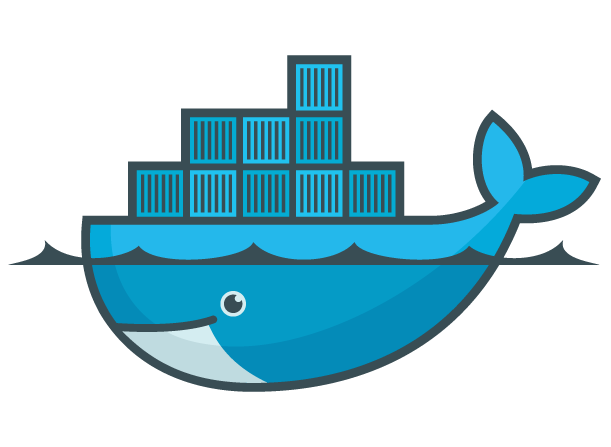
\includegraphics[scale=0.4,right]{docker.png}}
\end{frame}

%-=-=-=-=-=-=-=-=-=-=-=-=-=-=-=-=-=-=-=-=-=-=-=-=
%
%	SECTION: BACKGROUND
%
%-=-=-=-=-=-=-=-=-=-=-=-=-=-=-=-=-=-=-=-=-=-=-=-=

\section{Motivación}
\begin{frame}{Erase una vez...}
	\begin{figure}
		\centering
\includegraphicscopyright[width=\textwidth,height=0.8\textheight,keepaspectratio]{images/another}{Imagen: docker.com}
	\end{figure}
\end{frame}

\begin{frame}{Erase una vez...}
	\begin{figure}
		\centering
\includegraphicscopyright[width=\textwidth,height=0.8\textheight,keepaspectratio]{images/r_container}{Imagen: docker.com}	\end{figure}
\end{frame}


\begin{frame}{Hoy}
	\begin{figure}
		\centering
\includegraphicscopyright[width=\textwidth,height=0.8\textheight,keepaspectratio]{images/matrix}{Imagen: docker.com}	\end{figure}
\end{frame}


\begin{frame}{Hoy}
	\begin{figure}
		\centering
\includegraphicscopyright[width=\textwidth,height=0.8\textheight,keepaspectratio]{images/eliminates-matrix-from-hell}{Imagen: docker.com}
	\end{figure}
\end{frame}

\begin{frame}{Docker containers}
	\begin{figure}
		\centering
\includegraphicscopyright[width=\textwidth,height=0.8\textheight,keepaspectratio]{images/shipping-container-for-code}{Imagen: docker.com}
	\end{figure}
\end{frame}


%-=-=-=-=-=-=-=-=-=-=-=-=-=-=-=-=-=-=-=-=-=-=-=-=
%
%	SECTION: STRUCTURE
%
%-=-=-=-=-=-=-=-=-=-=-=-=-=-=-=-=-=-=-=-=-=-=-=-=
\section{Docker}

\begin{frame}{Docker}
	\begin{itemize}
		\item Docker es un proyecto open-source
		\item Utiliza la tecnología de los containers (libcontainer).
		\item Para ``construir, migrar y correr aplicaciones distribuidas".
	\end{itemize}

\end{frame}

\begin{frame}{¿Qué son los containers?}
	\begin{itemize}
		\item ¿Qué son los containers?
			\begin{itemize}
				\item Desde lejos, parecen ser como VM.
				\item Puedo instalar aplicaciones, permisos root, red filesystems, etc.
				\item Pero son ambientes virtuales livianos, rápidos de iniciar (boot en ms), fácil de migrar, reproducibles y aislados.
			\end{itemize}
	\end{itemize}
\end{frame}


\begin{frame}{}
	\begin{figure}
		\centering
		\includegraphicscopyright[width=\linewidth]{images/container_vs_vm.jpg}{\href{http://www.qafe.com/what-is-docker-why-en-how-use-it/}{qafe.com}}
	\end{figure}
\end{frame}

\begin{frame}{Docker containers}

\begin{itemize}
	\item Las aplicaciones corren en los containers.
\end{itemize}
	
	
	\begin{exampleblock}{Iniciar un container}
		\$ docker run [OPTIONS] IMAGE [COMMAND] arg\\
		\$ docker run -d ubuntu apache2ctl
	\end{exampleblock}
\end{frame}


\begin{frame}{Docker image}
\begin{itemize}
	\item Template read-only se obtienen:
	\begin{itemize}
		\item Repositorio público o privado
		\item Construidas por Dockerfile
	\end{itemize}
	\item Son usadas para construir Docker containers.
	\item Los cambios realizados se hacen a través de capas.
\end{itemize}
\begin{figure}[H]
  \centering
  \includegraphicscopyright[width=0.5\textwidth]{images/docker-filesystems-multilayer}{Imagen: docker.com}
\end{figure}	
\end{frame}


\begin{frame}[containsverbatim]{DOCKERFILE}
\begin{lstlisting}
FROM ubuntu
MAINTAINER Maximiliano Osorio
RUN apt-key adv --keyserver keyserver.ubuntu.com --recv 7F0CEB10
RUN echo "deb http://downloads-distro.mongodb.org/repo/ubuntu-upstart dist 10gen" | tee -a /etc/apt/sources.list.d/10gen.list
RUN apt-get update
RUN apt-get -y install apt-utils
RUN apt-get -y install mongodb-10gen
CMD ["/usr/bin/mongod", "--config", "/etc/mongodb.conf"] 
\end{lstlisting}
\end{frame}




\begin{frame}{Docker registry}
\begin{itemize}
	\item Repositorios públicos (Docker Hub) y privados de imágenes.
	\item Permite subir y bajar imágenes con sistemas operativos o aplicaciones ya configuradas.
	\item Imágenes son verificadas autenticidad y integridad.	
\end{itemize}
\end{frame}


\begin{frame}{Docker registry}

\begin{figure}[H]
  \centering
  \includegraphicscopyright[width=\textwidth,height=0.8\textheight,keepaspectratio]{images/registry-dynamic.png}{http://cloud.51cto.com/}
    \label{fig:dynamic}
\end{figure}	
\end{frame}


\begin{frame}{Aislamiento}
	\begin{itemize}
		\item \textbf{Limite de recursos:}  Cgroups controlan la cantidad de recursos como CPU, memoria y disk I/O.
		\item \textbf{Process:} Utiliza PID namespaces (kernel \(\geq 2.6.32\)), el container solo puede ver los procesos del container.
		\item \textbf{Filesystem:} Mismo mecanismo y mismo resultado que con los procesos. Existen filesystem que deben ser montados (ej. /sys).
		\item \textbf{Device:} Cgroups permite usar algunos devices \footnote{/dev/console, /dev/null, /dev/zero, /dev/full, /dev/tty*, /dev/urandom, /dev/random, /dev/fuse} y bloquea la posibilidad de crear y usar otros devices.
		\item \textbf{IPC:} Los procesos corriendo en los containers utilizan \textit{IPC namespaces} que permite la creación de un \textit{IPC} separado y independiente para cada container 
	\end{itemize}
\end{frame}

\begin{frame}{Aislamiento}
	\begin{itemize}
	
		\item \textbf{Network:}
		Para cada container, Docker crea una red independiente usando \textit{network namespaces}, compuesta de su propia IP, rutas, \textit{network devices}.
		Por defecto, la conexión se realiza gracias al host que provee un \textit{Virtual Ethernet bridge} en la máquina, llamado docker0 que automáticamente realiza un \textit{forward} de los paquetes entre las interfaces del container.
	\end{itemize}
	
	\begin{figure}[H]
  \centering
  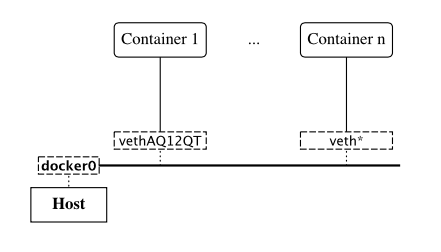
\includegraphics[width=0.5\textwidth]{images/network.png}
    \label{fig:dynamic}
\end{figure}	
\end{frame}

\subsection{Beneficios}

\begin{frame}{Beneficios}
	\begin{itemize}
		\item Despliegue rápido de aplicaciones: Los requerimientos son mínimos por lo que se reduce el tamaño y por lo tanto el despliegue es rápido.
		\item Portabilidad: La aplicación y todas las dependencias quedan en el container que es independiente al kernel o plataforma.
		\item Ambiente reproducible: La aplicación se comportará de la misma manera en otro host.
		\item Control de versión: Inspeccionar diferencias y hacer rollbacks.
		\item Re uso de componentes: Re usa capas anteriores lo cual lo hace más liviano.
		\item Compartir: Se puede utilizar repositorios públicos o privados de imágenes ya configuradas.
		\item Escalabilidad.
	\end{itemize}
\end{frame}

\subsection{Rendimiento}



\begin{frame}{Pruebas}

An updated performance comparison of virtual machines and linux containers \cite{felter2014updated}
\begin{itemize}
	\item CPU-PXZ: PXZ es utilidad de compresión en paralelo. 
	\item HPC - Linpack: Limpack soluciona un sistema de ecuaciones lineales usando un algoritmo de factorización LU.
	\item Memory bandwidth - Stream: Un programa para benchmarking que hace operaciones simples sobre vectores.
	\item Random Memory Access: Estrés de forma aleatoria a la memoria 
\end{itemize}
\end{frame}

\begin{frame}{Resultados}
\begin{table}[h]
\centering
\resizebox{\textwidth}{!}{%
\begin{tabular}{|l|l|l|l|l|l|}
\hline
Workload &  & Native & Docker & KVM-untuned & KVM-tuned \\ \hline
PXZ (MB/s) &  & 76.2 & 73.5 (-4\%) & 59.2 (-22\%) & 62.2 (-18\%) \\ \hline
Linpack (GFLOPS) &  & 290.8 & 290.9 (-0\%) & 241.3 (-17\%) & 284.2 (-2\%)\\ \hline
RandomAccess (GUPS) &  & 0.0126 & 0.0124 (-2\%)  & 0.0125 (-1\%) & \multirow{5}{*}{Tuned run not warranted} \\ \cline{1-5}
\multirow{4}{*}{Stream (GB/s)} & Add & 45.8 & 45.6 (-0\%) & 45.0 (-2\%) &  \\ \cline{2-5}
 & Copy & 41.3  & 41.2 (-0\%)  & 40.1 (-3\%) &  \\ \cline{2-5}
 & Scale & 41.2 & 41.2 (-0\%)  & 40.0 (-3\%)  &  \\ \cline{2-5}
 & Triad & 45.6  & 45.6 (-0\%)  & 45.0 (-1\%)  &  \\ \hline
\end{tabular}
}
\caption{Resultados}

\end{table}
\end{frame}


\begin{frame}{Latencia}
	\begin{itemize}
		\item Dos máquinas idénticas conectadas por 10Gbps Ethernet.
		\item Cliente envia un paquete 100-byte.
		\item Servidor responde con un paquete 200-byte.
	\end{itemize}
\begin{figure}[H]
  \centering
  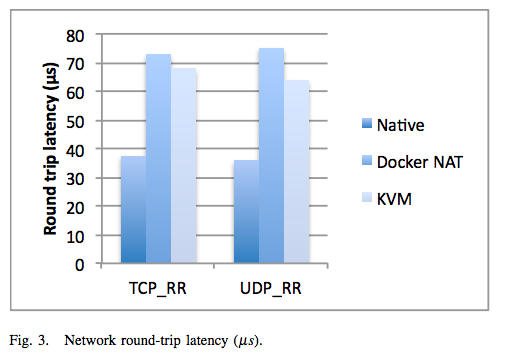
\includegraphics[width=0.9\textwidth]{images/latency.png}
    \caption{Network}
    \label{fig:dynamic}
\end{figure}	
\end{frame}

\begin{frame}{Block I/O}
	\begin{itemize}
		\item 20 TB IBM FlashSystem 840 flash SSD
		\item 8 Gbps Fibre Channel links
	\end{itemize}
\begin{figure}[H]
  \centering
  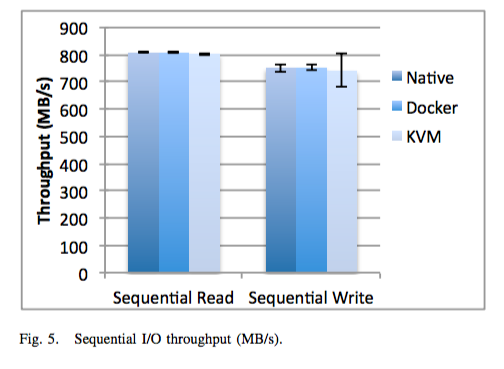
\includegraphics[width=0.9\textwidth]{images/block}
    \label{fig:dynamic}
\end{figure}	
\end{frame}

\begin{frame}{Block I/O}
	\begin{itemize}
		\item 20 TB IBM FlashSystem 840 flash SSD
		\item 8 Gbps Fibre Channel links
	\end{itemize}
\begin{figure}[H]
  \centering
  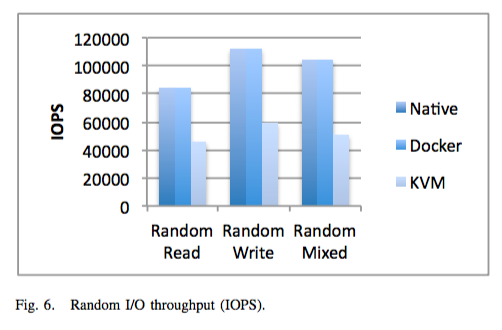
\includegraphics[width=0.9\textwidth]{images/block2}
    \label{fig:dynamic}
\end{figure}	
\end{frame}


\begin{frame}{mySQL}
\begin{itemize}
	\item SysBench
	\item Base de datos de 2 millones de registros.
	\item Operaciones: SELECT, 2 UPDATES, DELETE, INSERT
\end{itemize}

\begin{table}[h]
\centering
\begin{tabular}{|l|l|l|}
\hline
Configuration & Network & Storage \\ \hline
Native & Native & Native \\ \hline
Docker net=host Volume & Native & Native \\ \hline
Docker NAT Volume & NAT & Native \\ \hline
Docker NAT AUFS & NAT & AUFS \\ \hline
KVM & vhost-net & virtio + qcow \\ \hline
\end{tabular}
\caption{mysql configurations}
\label{my-label}
\end{table}


\end{frame}

\begin{frame}{mySQL}

  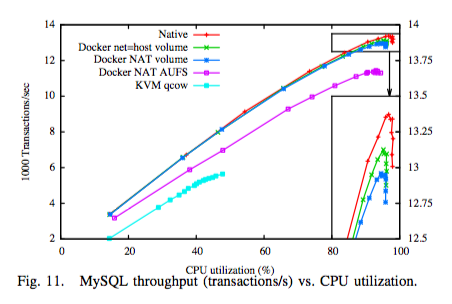
\includegraphics[width=0.9\textwidth]{images/mysql1}
\end{frame}
\begin{frame}{mySQL}

  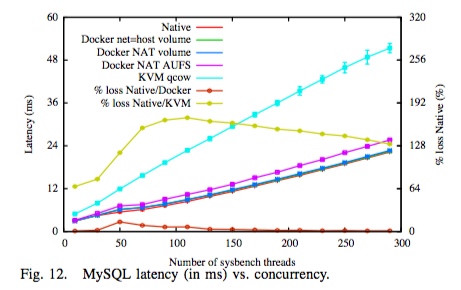
\includegraphics[width=0.9\textwidth]{images/mysql2}
\end{frame}



\begin{frame}{Infiniband}
	\begin{itemize}
		\item  Sin Docker-nat
	\end{itemize}
\begin{figure}[H]
  \centering
  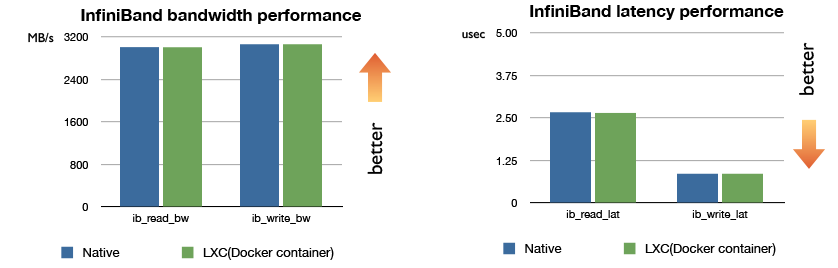
\includegraphics[width=1\textwidth]{images/infiniband.png}
    \label{fig:dynamic}
\end{figure}	
\end{frame}


\begin{frame}{Comunidad}
\begin{figure}[H]
  \centering
  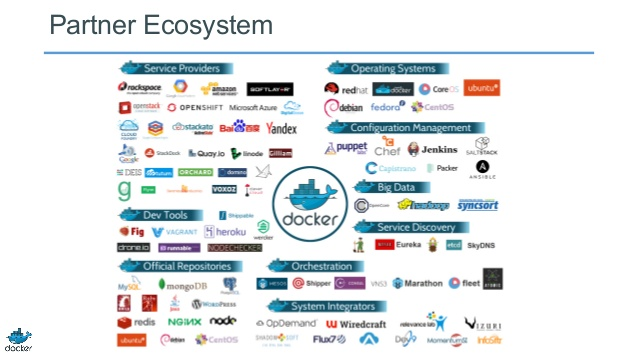
\includegraphics[width=1\textwidth]{images/ecosystem.jpg}
    \label{fig:dynamic}
\end{figure}		
\end{frame}
	
\section*{Referencias}
\begin{frame}{Referencias}
	\begin{thebibliography}{10}
    
	\beamertemplatebookbibitems
	\bibitem{felter2014updated}
	An updated performance comparison of virtual machines and linux containers
	\newblock Felter, Wes and Ferreira, Alexandre and Rajamony, Ram and Rubio, Juan
	\newblock 2014
  \end{thebibliography}
\end{frame}

\maketitle

\section{Demos}
\begin{frame}{demo}
\begin{figure}[H]
  \centering
  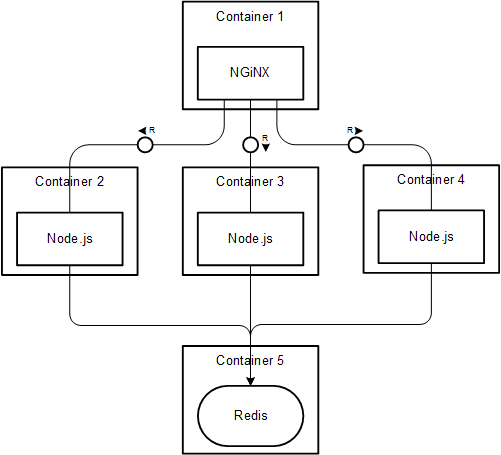
\includegraphics[width=0.8\textwidth]{images/DockerSample.png}
    \label{fig:dynamic}
\end{figure}	
\end{frame}

\end{document}